%gibt an: Papierformat, Schriftgr��e
\documentclass[a4paper,german,12pt]{article}
\setlength{\parskip}{0.2cm}
\setlength{\parindent}{0cm}
%-----------------------------------------------------------------------------------------------------------------------------
%�bersetzung von E in D
\usepackage{german}
%Einstellung der Randabst�nde
\usepackage[lmargin={2.5cm},rmargin={2.5cm},tmargin={1.5cm},bmargin={2.5cm}]{geometry}
%zur Einbindung von Graphiken
\usepackage{graphicx}
%Bearbeitung von Kopf- und Fusszeile
\usepackage{fancyhdr}
%Schriftart
\usepackage{helvet}
%stellt unabh�ngige Textmarken zu Verf�gung
\usepackage{extramarks}
%aktiviert eine Umgebung in der der Mathematikmodus aktiv ist
\usepackage{amsmath}
%aktiviert eine Umgebung in der der Mathematikmodus aktiv ist
\usepackage{amsthm}
%aktiviert eine Umgebung in der der Mathematikmodus aktiv ist
\usepackage{amssymb}
%aktiviert Hyperlinks
\usepackage{hyperref} 
%Stellt das Eurozeichen � zu Verf�gung
\usepackage[right]{eurosym}
%�bersetzt die Tastatureingaben f�r LaTex
\usepackage[latin1]{inputenc}
\usepackage{fancybox}
\usepackage{xcolor}
\usepackage{color}
\usepackage{float}
\usepackage{framed}
\usepackage{url}

%Weitere
\usepackage{bibgerm} %Bibliothek

\usepackage{booktabs}
\usepackage{tabularx} %Tabellen, die sich der Seitenbreite anpassen

\usepackage{multirow} % Verbundene Zellen in Tabellen

\usepackage{rotating} % Quergestellte Tabellen
\usepackage{rotfloat}

\usepackage[bottom]{footmisc} %Fu�noten immer am Ende der Seite

%Definitionen

\newtheoremstyle{mystyle}% name
{10pt}% Space above
{10pt}% Space below
{\itshape}% Body font
{}% Indent amount: 
{\bfseries}% Theorem head font
{:}% Punctuation after theorem head
{0.5em}% Space after theorem head
{\thmname{#1}\thmnumber{ #2}:\thmnote{ #3}}% Theorem head 

\theoremstyle{mystyle}% default
\newtheorem{definition}{Definition}
\numberwithin{equation}{section}
\renewcommand{\proofname}{Beweis}

%Paragraphen

\newcommand{\myparagraph}[1]{\paragraph{}\mbox{}\\}


%-----------------------------------------------------------------------------------------------------------------------------------------
\renewcommand{\baselinestretch}{1.2}
\fancyhead[LO]{\slshape \small \firstleftmark}
\fancyhead[RO]{\normalsize\thepage} \fancyfoot{}
\begin{document}
%-----------------------------------------------------------------------------------------------------------------------------------------
%Titelseite

\begin{titlepage}
% font / Schriftart
%------------------	
\begin{figure}[htbp]
  %\centering
  \begin{minipage}[t]{0.4\textwidth} 
    
\includegraphics[scale=0.75]{0_Logos/kit.jpg}  
    
  \end{minipage}
  \hfill
  \begin{minipage}[b]{0.3\textwidth} 
	\begin{flushleft}
		
\includegraphics[scale=0.09]{0_Logos/aifb.png}     
	\end{flushleft}
	\begin{flushleft}
		\tiny\textbf{Institut f�r Angewandte Informatik}
		\textbf{und Formale Beschreibungsverfahren}
	\end{flushleft}
  \end{minipage}
\end{figure}

\vspace*{1.5cm}
\leftskip=4cm
		\textbf{{\Huge %TODO
		Titel der Abschlussarbeit}\\
		{\Huge %TODO 
		[auch mehrzeilig m�glich]}}
		\vspace*{1.5cm}\\
		{\Large %TODO
		Abschluss-/Studienarbeit}\\
		{\Large von} \\
		{\Large %TODO
		Vorname Nachname}
		\vspace*{3.5cm}\\
		an der Fakult�t f�r Wirtschaftswissenschaften
		\vspace*{0.5cm}\\
		In dem Studiengang\\
		%TODO
		Name Studiengang
		\vspace*{1.5cm}\\
		eingereicht am %TODO Datum
		beim\\
		Institut f�r Angewandte Informatik\\
		und Formale Beschreibungsverfahren\\
		des Karlsruher Instituts f�r Technologie
		\vspace*{2.5cm}\\
		Referent: Prof. Dr. %TODO Referent
		\\
		Betreuer: %TODO Betreuer
		\vspace*{1.5cm}\\
		{\footnotesize KIT -- Universit�t des Landes Baden-W�rttemberg und}\\
		{\footnotesize nationales Forschungszentrum in der Helmholtz-Gemeinschaft}\\
		\hfill

\end{titlepage}


\thispagestyle{empty}\cleardoublepage

\mbox{}\thispagestyle{empty}
\cleardoublepage

\mbox{}\thispagestyle{empty}

\vspace*{1cm}

{\Large \textbf{Eidesstattliche Erkl�rung}} 

\bigskip

Ich versichere hiermit wahrheitsgem��, die Arbeit und alle Teile daraus selbst�ndig angefertigt, alle benutzten Hilfsmittel vollst�ndig und genau angegeben und alles kenntlich gemacht zu haben, was aus Arbeiten anderer unver�ndert oder mit Ab�nderung entnommen wurde.\\

\vspace{1cm}
 
\textit{Karlsruhe, den DATUM} \hspace{4cm} \textit{NAME} \\

\thispagestyle{empty}\cleardoublepage

\mbox{}\thispagestyle{empty}
\cleardoublepage
\rmfamily \pagestyle{fancy} \setcounter{secnumdepth}{4}


\pagenumbering{roman}
\setcounter{page}{3} 
\tableofcontents
\newcounter{roemisch} 
\setcounter{roemisch}{\value{page}}
\markboth{ABK�RZUNGSVERZEICHNIS}{Abk�rzungsverzeichnis}
\section*{Abk�rzungsverzeichnis}
\begin{table}[h]
    \begin{tabular}{rl}
    NILM & Non-intrusive load monitoring\\
    KNN & K�nstliches Neuronale Netz\\
    ESHL & Energy Smart Home Lab\\
    MLP & Multi Layer Perceptron\\
    \end{tabular}%
\end{table}%

\cleardoublepage
\listoffigures
\cleardoublepage
\listoftables
\cleardoublepage

\setcounter{page}{2} \pagenumbering{arabic}

\interfootnotelinepenalty=10000 % Keine Seitenumbr�che bei Fu�noten

 % % % % % % % % % % % % %INHALTE % % % % % % % % % % % % % %
 \section{Einleitung}
\label{Einleitung}

%\subsection{Motivation}
%\label{Motivation}
	Energie zu sparen ist seit Langem ein Ziel der Umweltpolitik, dennoch steigt der Energieverbrauch in Industriel"andern kontinuierlich und es werden nach wie vor Wege gesucht, diesen zu senken. 
	In den USA verursachen private Haushalte 40\% des CO2-Aussto{\ss}es \cite{vandenbergh2008individual} und stehen deshalb im Fokus vieler Programme zum Energiesparen. \\
	Je nach Studie besteht f"ur die Haushalte ein Einsparungspotential von bis zu 20\% \cite{armel2013disaggregation} f"ur dessen Energieverbrauch, Fischer \cite{fischer2008feedback} untersucht mehrere dieser Studien und beschreibt ein durchschnittliches Einsparungspotential von 5-12\%. 
	Um dieses Einsparungspotential auszunutzen, muss der Nutzer regelm"a{\ss}ig und m"oglichst genau "uber seinen Verbrauch aufgekl"art werden. 	%TODO Graphik Armel
	\begin{figure}[ht]
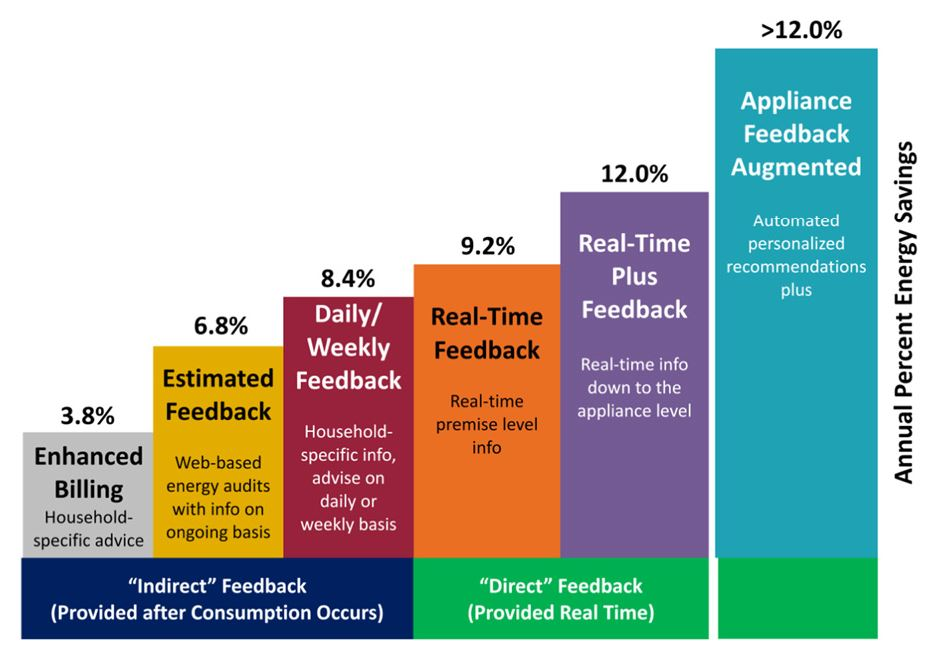
\includegraphics[width=\textwidth]{1_Grafiken/fig1armel.jpg}
	\caption[Einsparungpotentiale nach Ma{\ss}nahme]{Grafik zu Einsparpotetialen je nach getroffener Aufkl"arungsma{\ss}nahme aus \cite{armel2013disaggregation}}
\label{potentiale}
\end{figure}

	Er kann sich oft nicht mit seinem Verbrauch identifizieren, weil dieser intransparent und durch die langen Rechnungsintervalle nicht pr"asent ist. \\
	Damit der Nutzer anf"angt sich selbst zu kontrollieren, muss er begreifen, dass sich sein Verhalten auf seinen Verbrauch auswirkt und er ihn auch durch die gezielte Ver"anderungen seines Handelns senken kann \cite{fischer2008feedback}.\\
	Non-intrusive load monitoring (NILM) bietet nun die Chance dem Nutzer eine regelm"a{\ss}ige, detaillierte R"uckmeldung zu seinem Energiekonsum zu geben, Kolter und Matthew \cite{kolter2011redd} beschreibt NILM als die Aufgabe aus einem, f"ur den gesamten Haushalt messenden Stromz"ahler, R"uckschl"usse "uber die elektrische Last einzelner Ger"ate zu ziehen.
	Ein solches System wird dem Konsumenten helfen, verschwenderische Verhaltensweisen und Ger"ate zu identifizieren ohne den Haushalt mit vielen digitalen Z"ahlern f"ur die individuellen Ger"ate ausr"usten zu m"ussen, wie es derzeit z.B. mit sogenannten \textit{Energiekostenmessger"aten} auf Steckerbasis praktiziert wird.

\subsection{Fragestellung}
\label{Fragestellung}
 	Viele Systeme zur Disagregation oder zu verschiedenen Vorhersage-Aufgaben benutzen Ans"atze des Maschinellen Lernens. Sie ben"otigen annotierte (gelabelte) Trainingsdaten, um robuste Modelle zu erzeugen. Annotieren bedeutet in diesem Zusammenhang, die Daten mit Metadaten wie etwa dem Ger"atezustand zu versehen. Mehr Trainingsdaten f"uhren in der Regel zu besseren Modellen, die Annotation ist allerdings sehr aufw"andig, weil sie manuell erfolgen muss. Der Ansatzpunkt dieser Arbeit ist, das Problem der Disagregation auf ein Ger"at zu reduzieren und so zu vereinfachen. Nun kann man ein robustes Modell mit nur wenigen Trainingsdaten erstellen und mit diesem dann eine gro{\ss}e Menge an Daten schnell annotieren. Diese gelabelten Daten sollen dann wiederum als Trainingsdaten f"ur schwierigere Aufgaben verwendet werden. 
	Aufgabe dieser Bachelorarbeit ist es ein System zu entwickeln, welches in der Lage ist die Zust"ande von ausgew"ahlten Ger"aten in einem disaggregierten Lastgang zu klassifizieren und so eine Segmentierung f"ur diese Ger"ate zu erstellen. Dies beinhaltet sowohl die n"otige Vorverarbeitung der Daten sowie eventuelle nachtr"agliche Formatierungen. Die eigentliche Klassifikation soll mit K"unstlichen Neuronalen Netzen (KNN) stattfinden, dabei sollte eine m"oglichst hohe Akkurarit"at erreicht werden, da Systeme, die mit den resultierenden Daten trainiert werden keine M"oglichkeit haben Fehler, die bereits in den Trainingsdaten sind, zu korrigieren. 
Au{\ss}erdem soll versucht werden aus den klassifizierten Daten wieder einen Lastgang zu erstellen. Dies soll die M"achtigkeit der Segmentierung der Ger"atezust"ande untersuchen und feststellen ob man zuverl"assig den Lastgang des Ger"ats vorhersagen kann, wenn es seine Zustandsfolge im Voraus bekannt gibt. 

\subsection{Weiterer Aufbau}
\label{Weiterer Aufbau}
	Im folgenden Kapitel~\ref{Datensatz} werden die verwendeten, disaggregierten Energiedatens"atze beschrieben. Insbesondere werden die gemessenen Werte und die daraus berechenbaren Werte untersucht. 
	Kapitel~\ref{Vorverarbeitung} gibt zun"achst einen "Uberblick "uber die aktuelle Forschung im Bereich Vorverarbeitung der Daten und Feature-Auswahl, anschlie{\ss}end werden die f"ur diese Arbeit verwendeten Vorverarbeitungsschritte und Features erl"autert.
	In Kapitel~\ref{Klassifizierung} soll schlie{\ss}lich die eigentliche Klassifizierung beschrieben werden, hier werden insbesondere das verwendete Netz und die Trainingsmethoden besprochen. Auch hier wird es einen kurzen "Uberblick "uber die aktuelle Forschung geben.
	In Kapitel~\ref{Generierung} wird die Generierung eines Lastprofils aus dem Zustandsprofil erl"autert. Es wird ein Ansatz aus der aktuellen Forschung beschrieben und auf dieses Problem adaptiert. 
	In Kapitel~\ref{Evaluation} findet die Evaluation statt, hier werden verschiedene Klassifikationsaufgaben ausgef"uhrt und ausgewertet. 
	Am Schluss steht das Fazit in Kapitel~\ref{fazit}, in dem die Ergebnisse zusammengefasst und mit urspr"ungliche Fragestellung verglichen werden. 

 \section{Kapitel X}
\label{KapitelX}
Lorem ipsum dolor sit amet, consetetur sadipscing elitr, sed diam nonumy eirmod tempor invidunt ut labore et dolore magna aliquyam erat, sed diam voluptua. At vero eos et accusam et justo duo dolores et ea rebum. Stet clita kasd gubergren, no sea takimata sanctus est Lorem ipsum dolor sit amet. Lorem ipsum dolor sit amet, consetetur sadipscing elitr, sed diam nonumy eirmod tempor invidunt ut labore et dolore magna aliquyam erat, sed diam voluptua. At vero eos et accusam et justo duo dolores et ea rebum. Stet clita kasd gubergren, no sea takimata sanctus est Lorem ipsum dolor sit amet. Lorem ipsum dolor sit amet, consetetur sadipscing elitr, sed diam nonumy eirmod tempor invidunt ut labore et dolore magna aliquyam.

\subsection{Unterkapitel}
\label{Unterkapitel}
Lorem ipsum dolor sit amet, consetetur sadipscing elitr, sed diam nonumy eirmod tempor invidunt ut labore et dolore magna aliquyam erat, sed diam voluptua. At vero eos et accusam et justo duo dolores et ea rebum. Stet clita kasd gubergren, no sea takimata sanctus est Lorem ipsum dolor sit amet. Lorem ipsum dolor sit amet, consetetur sadipscing elitr, sed diam nonumy eirmod tempor invidunt ut labore et dolore magna aliquyam erat, sed diam voluptua. At vero eos et accusam et justo duo dolores et ea rebum. Stet clita kasd gubergren, no sea takimata sanctus est Lorem ipsum dolor sit amet. Lorem ipsum dolor sit amet, consetetur sadipscing elitr, sed diam nonumy eirmod tempor invidunt ut labore et dolore magna aliquyam erat, sed diam voluptua. At vero eos et accusam et justo duo dolores et ea rebum. Stet clita kasd gubergren, no sea takimata sanctus est Lorem ipsum dolor sit amet.   

  \begin{definition}[Begriff]
  \label{Begriff}
Lorem ipsum dolor sit amet, consetetur sadipscing elitr, sed diam 
  \end{definition}

Duis autem vel eum iriure dolor in hendrerit in vulputate velit esse molestie consequat, vel illum dolore eu feugiat nulla facilisis at vero eros et accumsan et iusto odio dignissim qui blandit praesent luptatum zzril delenit augue duis dolore te feugait nulla facilisi. Lorem ipsum dolor sit amet, consectetuer adipiscing elit, sed diam nonummy nibh euismod tincidunt ut laoreet dolore magna aliquam erat volutpat.\footnote{Lorem ipsum dolor sit amet, consetetur.}  

Ut wisi enim ad minim veniam, quis nostrud exerci tation (vgl. Kapitel \ref{Motivation} auf Seite \pageref{Motivation}) ullamcorper suscipit lobortis nisl ut aliquip ex ea commodo consequat. Duis autem vel eum iriure dolor in hendrerit in vulputate velit esse molestie consequat, vel illum dolore eu feugiat nulla facilisis at vero eros et accumsan et iusto odio dignissim qui blandit praesent luptatum zzril delenit augue duis dolore te feugait nulla facilisi.   

Nam liber tempor cum soluta nobis eleifend option congue nihil imperdiet doming id quod mazim placerat facer possim assum. Lorem ipsum dolor sit amet, consectetuer adipiscing elit, sed diam nonummy nibh euismod tincidunt ut laoreet dolore magna aliquam erat volutpat. Ut wisi enim ad minim veniam, quis nostrud exerci tation ullamcorper suscipit lobortis nisl ut aliquip ex ea commodo consequat (vgl. Abbildung \ref{IT_Architekturen}).  
\begin{figure}[H]
\begin{center}
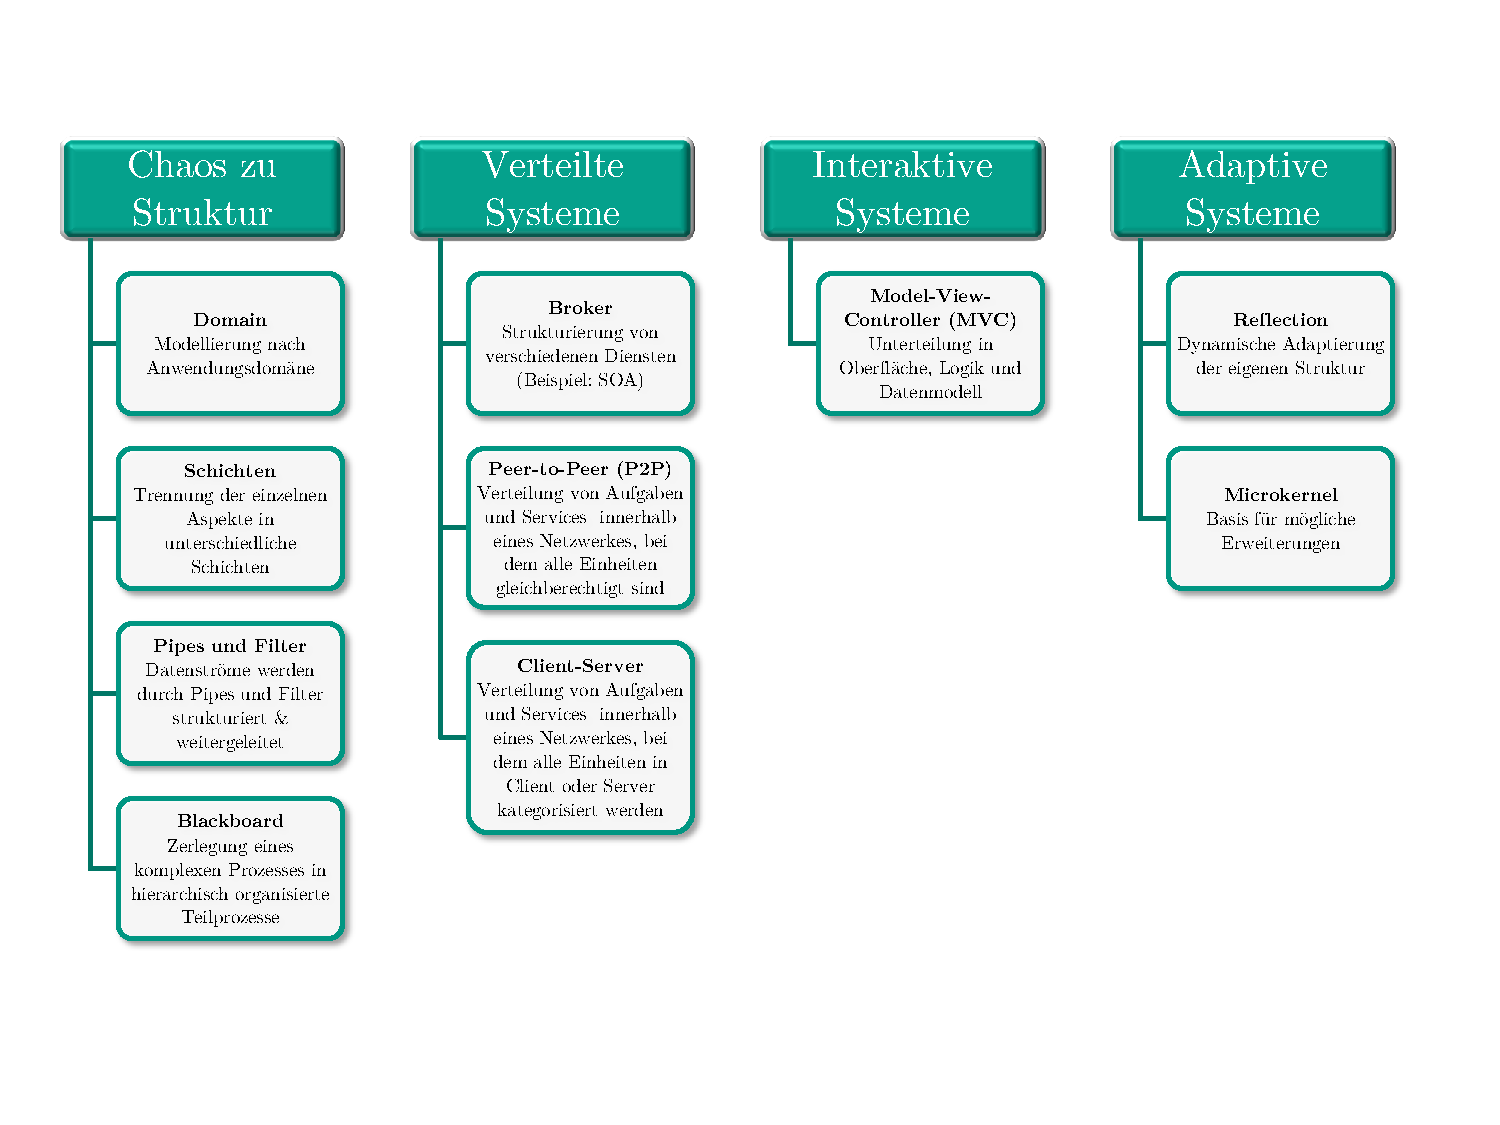
\includegraphics[width=0.8\textwidth]{1_Grafiken/architekturen.PDF}
\caption{IT-Architekturen, Eigene Darstellung auf Grundlage von  \cite{buschmann}}
 \label{IT_Architekturen}
\end{center}
\end{figure}
Duis autem vel eum iriure dolor in hendrerit in vulputate velit esse molestie consequat, vel illum dolore eu feugiat nulla facilisis.   

At vero eos et accusam et justo duo dolores et ea rebum. Stet clita kasd gubergren, no sea takimata sanctus est Lorem ipsum dolor sit amet. Lorem ipsum dolor sit amet, consetetur sadipscing elitr, sed diam nonumy eirmod tempor invidunt ut labore et dolore magna aliquyam erat, sed diam voluptua. At vero eos et accusam et justo duo dolores et ea rebum. Stet clita kasd gubergren, no sea takimata sanctus est Lorem ipsum dolor sit amet. Lorem ipsum dolor sit amet, consetetur sadipscing elitr, At accusam aliquyam diam diam dolore dolores duo eirmod eos erat, et nonumy sed tempor et et invidunt justo labore Stet clita ea et gubergren, kasd magna no rebum. sanctus sea sed takimata ut vero voluptua. est Lorem ipsum dolor sit amet. Lorem ipsum dolor sit amet, consetetur sadipscing elitr, sed diam nonumy eirmod tempor invidunt ut labore et dolore magna aliquyam erat (siehe Tabelle \ref{Speiseplan_der_Raupe_Nimmersatt}).   

% Der Befehl tabular definiert die tabular-Umgebung, die zur Erzeugung von Tabellen dient.  Gibt man als Position t an, dann dient die oberste Zeile der Tabelle als Verankerung, bei b dagegen die unterste Zeile. Spalten enth�lt f�r jede Spalte einen der Buchstaben l (linksb�ndig), c (zentriert) oder r (rechtsb�ndig). Zus�tzlich kann man mittels | einen senkrechten Trennstrich zwischen zwei Spalten einf�gen. Im Tabellenrumpf wird der Inhalt zweier Spalten durch & abgegrenzt, die Zeilen werden mit \\ beendet. Der Befehl table erm�glicht unter anderem das Einbinden einer Tabellenunterschrift und das Zentrieren der Tabelle auf der Seitenmitte.

\begin{table}[h]
\centering
\begin{tabular}{|l|l|l|}
\hline
Montag & Dienstag & Mittwoch\\
\hline
Apfel & Birne & Pflaume\\
\hline
\end{tabular}
\caption{Speiseplan der Raupe Nimmersatt}
\label{Speiseplan_der_Raupe_Nimmersatt}
\end{table}

Consetetur sadipscing elitr, sed diam nonumy eirmod tempor invidunt ut labore et dolore magna aliquyam erat, sed diam voluptua. At vero eos et accusam et justo duo dolores et ea rebum. Stet clita kasd gubergren, no sea takimata sanctus est Lorem ipsum dolor sit amet. Lorem ipsum dolor sit amet, consetetur sadipscing elitr, sed diam nonumy eirmod tempor invidunt ut labore et dolore magna aliquyam erat, sed diam voluptua. At vero eos et accusam et justo duo dolores et ea rebum. Stet clita kasd gubergren, no sea takimata sanctus est Lorem ipsum dolor sit amet. Lorem ipsum dolor sit amet, consetetur sadipscing elitr, sed diam nonumy eirmod tempor invidunt ut labore et dolore magna aliquyam erat, sed diam voluptua. At vero eos et accusam et justo duo dolores et ea rebum. Stet clita kasd gubergren, no sea takimata sanctus.   

Lorem ipsum dolor sit amet, consetetur sadipscing elitr, sed diam nonumy eirmod tempor invidunt ut labore et dolore magna aliquyam erat, sed diam voluptua. At vero eos et accusam et justo duo dolores et ea rebum. Stet clita kasd gubergren, no sea takimata sanctus est Lorem ipsum dolor sit amet. Lorem ipsum dolor sit amet, consetetur sadipscing elitr, sed diam nonumy eirmod tempor invidunt ut labore et dolore magna aliquyam erat, sed diam voluptua. At vero eos et accusam et justo duo dolores et ea rebum. Stet clita kasd gubergren, no sea takimata sanctus est Lorem ipsum dolor sit amet. Lorem ipsum dolor sit amet, consetetur sadipscing elitr, sed diam nonumy eirmod tempor invidunt ut labore et dolore magna aliquyam erat, sed diam voluptua. At vero eos et accusam et justo duo dolores et ea rebum. Stet clita kasd gubergren, no sea takimata sanctus est Lorem ipsum dolor sit amet.   

\subsection{Weiteres Unterkapitel}
\label{Weiteres_Unterkapitel}
Duis autem vel eum iriure dolor in hendrerit in vulputate velit esse molestie consequat, vel illum dolore eu feugiat nulla facilisis at vero eros et accumsan et iusto odio dignissim qui blandit praesent luptatum zzril delenit augue duis dolore te feugait nulla facilisi. Lorem ipsum dolor sit amet, consectetuer adipiscing elit, sed diam nonummy nibh euismod tincidunt ut laoreet dolore magna aliquam erat volutpat.   

Ut wisi enim ad minim veniam, quis nostrud exerci tation ullamcorper suscipit lobortis nisl ut aliquip ex ea commodo consequat. Duis autem vel eum iriure dolor in hendrerit in vulputate velit esse molestie consequat, vel illum dolore eu feugiat nulla facilisis at vero eros et accumsan et iusto odio dignissim qui blandit praesent luptatum zzril delenit augue duis dolore te feugait nulla facilisi.   

Nam liber tempor cum soluta nobis eleifend option congue nihil imperdiet doming id quod mazim placerat facer possim assum. Lorem ipsum dolor sit amet, consectetuer adipiscing elit, sed diam nonummy nibh euismod tincidunt ut laoreet dolore magna aliquam erat volutpat. Ut wisi enim ad minim veniam, quis nostrud exerci tation ullamcorper suscipit lobortis nisl ut aliquip ex ea commodo

  
\subsection{Zus�tzliches Unterkapitel}
\label{Zusaetzliches_Unterkapitel}
Consetetur sadipscing elitr, sed diam nonumy eirmod tempor invidunt ut labore et dolore magna aliquyam erat, sed diam voluptua. At vero eos et accusam et justo duo dolores et ea rebum. Stet clita kasd gubergren, no sea takimata sanctus est Lorem ipsum dolor sit amet. Lorem ipsum dolor sit amet, consetetur sadipscing elitr, sed diam nonumy eirmod tempor invidunt ut labore et dolore magna aliquyam erat, sed diam voluptua. At vero eos et accusam et justo duo dolores et ea rebum. Stet clita kasd gubergren, no sea takimata sanctus est Lorem ipsum dolor sit amet. Lorem ipsum dolor sit amet, consetetur sadipscing elitr, sed diam nonumy eirmod tempor invidunt ut labore et dolore magna aliquyam erat, sed diam voluptua. At vero eos et accusam et justo duo dolores et ea rebum. Stet clita kasd gubergren, no sea takimata sanctus.   

Lorem ipsum dolor sit amet, consetetur sadipscing elitr, sed diam nonumy eirmod tempor invidunt ut labore et dolore magna aliquyam erat, sed diam voluptua. At vero eos et accusam et justo duo dolores et ea rebum. Stet clita kasd gubergren, no sea takimata sanctus est Lorem ipsum dolor sit amet. Lorem ipsum dolor sit amet, consetetur sadipscing elitr, sed diam nonumy eirmod tempor invidunt ut labore et dolore magna aliquyam erat, sed diam voluptua. At vero eos et accusam et justo duo dolores et ea rebum. Stet clita kasd gubergren, no sea takimata sanctus est Lorem ipsum dolor sit amet. Lorem ipsum dolor sit amet, consetetur sadipscing elitr, sed diam nonumy eirmod tempor invidunt ut labore et dolore magna aliquyam erat, sed diam voluptua. At vero eos et accusam et justo duo dolores et ea rebum. Stet clita kasd gubergren, no sea takimata sanctus est Lorem ipsum dolor sit amet.   



 \section{Fazit}
\label{fazit}
Lorem ipsum dolor sit amet, consetetur sadipscing elitr, sed diam nonumy eirmod tempor invidunt ut labore et dolore magna aliquyam erat, sed diam voluptua. At vero eos et accusam et justo duo dolores et ea rebum. Stet clita kasd gubergren, no sea takimata sanctus est Lorem ipsum dolor sit amet. Lorem ipsum dolor sit amet, consetetur sadipscing elitr, sed diam nonumy eirmod tempor invidunt ut labore et dolore magna aliquyam erat, sed diam voluptua. At vero eos et accusam et justo duo dolores et ea rebum. Stet clita kasd gubergren, no sea takimata sanctus est Lorem ipsum dolor sit amet. Lorem ipsum dolor sit amet, consetetur sadipscing elitr, sed diam nonumy eirmod tempor invidunt ut labore et dolore magna aliquyam erat, sed diam voluptua. At vero eos et accusam et justo duo dolores et ea rebum. Stet clita kasd gubergren, no sea takimata sanctus est Lorem ipsum dolor sit amet.   

Duis autem vel eum iriure dolor in hendrerit in vulputate velit esse molestie consequat, vel illum dolore eu feugiat nulla facilisis at vero eros et accumsan et iusto odio dignissim qui blandit praesent luptatum zzril delenit augue duis dolore te feugait nulla facilisi. Lorem ipsum dolor sit amet, consectetuer adipiscing elit, sed diam nonummy nibh euismod tincidunt ut laoreet dolore magna aliquam erat volutpat.   

Ut wisi enim ad minim veniam, quis nostrud exerci tation ullamcorper suscipit lobortis nisl ut aliquip ex ea commodo consequat. Duis autem vel eum iriure dolor in hendrerit in vulputate velit esse molestie consequat, vel illum dolore eu feugiat nulla facilisis at vero eros et accumsan et iusto odio dignissim qui blandit praesent luptatum zzril delenit augue duis dolore te feugait nulla facilisi.   

Nam liber tempor cum soluta nobis eleifend option congue nihil imperdiet doming id quod mazim placerat facer possim assum. Lorem ipsum dolor sit amet, consectetuer adipiscing elit, sed diam nonummy nibh euismod tincidunt ut laoreet dolore magna aliquam erat volutpat. Ut wisi enim ad minim veniam, quis nostrud exerci tation ullamcorper suscipit lobortis nisl ut aliquip ex ea commodo consequat.   

Duis autem vel eum iriure dolor in hendrerit in vulputate velit esse molestie consequat, vel illum dolore eu feugiat nulla facilisis.   

At vero eos et accusam et justo duo dolores et ea rebum. Stet clita kasd gubergren, no sea takimata sanctus est Lorem ipsum dolor sit amet. Lorem ipsum dolor sit amet, consetetur

% % % % % % % % % % % % % ANHANG% % % % % % % % % % % % % % % % 
\appendix %Anhang
 \section{Anhang}
\label{Anhang}

 %Anhang

% % % % % % % % % % % % % LITERATUR% % % % % % % % % % % % % % %
\bibliographystyle{geralpha} %Literaturverzeichnis
 \bibliography{Thesis} %Literaturverzeichnis
\end{document}
